\pdfminorversion=4
\documentclass[a4paper,12pt]{article}
\usepackage [spanish]{babel} 
\usepackage[utf8]{inputenc}
\usepackage{amsmath}
\usepackage{graphicx}
\usepackage{framed}
\usepackage{url}
\usepackage[makeroom]{cancel}

\usepackage{fancyhdr}

\newcommand{\ihat}{\hat{\textbf{\i}}}
\newcommand{\jhat}{\hat{\textbf{\j}}}
\newcommand{\khat}{\hat{\textbf{k}}}
\newcommand{\vol}{\mathop{\ooalign{\hfil$V$\hfil\cr\kern0.08em--\hfil\cr}}\nolimits}

\graphicspath{{../img/}}
 
\pagestyle{fancy}
\setlength\headheight{1.5cm}
\fancyhf{}
\rhead{
\includegraphics[width=3.0cm]{logo-mec.png}}
\lhead{
\includegraphics[width=3.5cm]{logo-utfsm.png}}
\renewcommand{\footrulewidth}{0.5pt}
\rfoot{\tiny{Departamento de Ingenier\'ia Mec\'anica}}
\lfoot{\tiny{Universidad T\'ecnica Federico Santa Mar\'ia}}

\title{Clase 8 --- Introducción a capa límite.} 
\author{Christopher Cooper}
\date{}

\begin{document}
\maketitle
\begin{framed}

Objetivos:
\begin{itemize}
    \item Modelar el efecto de la viscosidad en flujos cercanos a una pared.
    \item Mostrar las distintas definiciones de capa límite.
    \item Encontrar expresiones para las distintas definiciones de capa límite a partir de un perfil dado. 
\end{itemize}

Contenidos:
\begin{itemize}
    \item Flujo viscoso sobre una placa plana.
    \item La capa límite y su espesor.
    \item El espesor de desplazamiento.
    \item El espesor de momentum.
    \item El análisis de von Kármán.
\end{itemize}

Bibliografía:
\begin{itemize}
    \item White, F. M. (2008) Mecánica de Fluidos. McGraw-Hill. Sexta edición. Secciones 7.1-7.4
    \item Fox, R. W., Pritchard, P. J. y McDonald, A. T. (2009) Introduction to Fluid Mechanics. John Wiley \& Sons. Secciones 9.1-9.3
\end{itemize}
\end{framed}

\section*{Flujo viscoso sobre una superficie}

Hace algunas clases estuvimos estudiando flujo potencial, el cual era no viscoso.
Una implicancia de su ``no viscosidad'' era que la condición de borde en una pared era de impermeabilidad ($\mathbf{V}\cdot\mathbf{n}=0$), sin embargo, el flujo podía deslizarse.
Obviamente, sabemos que no existe tal cosa como un flujo ``no viscoso''. 
De hecho, experimentalmente podemos ver que la velocidad del fluido en la interfaz con el sólido es igual a la velocidad del sólido, en otras palabras, el fluido no desliza.
%
\begin{figure}[!h]
\centering
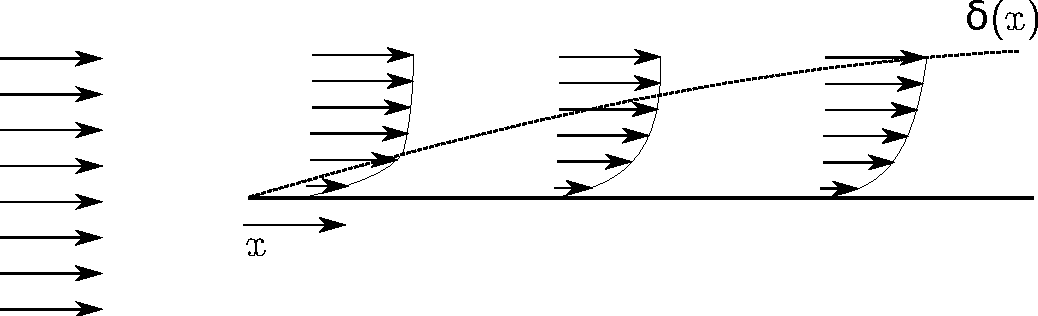
\includegraphics[width=0.8\textwidth]{clase04/capa_limite.pdf}
\caption{Flujo sobre una placa plana.}
\label{fig:capa_limite}
\end{figure}
%
Tomemos, por ejemplo, el flujo uniforme que se topa con una placa plana en la Figura \ref{fig:capa_limite}.
Lo que esperamos que ocurra es que el flujo en la placa tenga velocidad cero, y de ahí vaya creciendo paulatinamente hasta llegar a la velocidad de entrada $U_\infty$.
En el principio de la placa (a $x$ pequeño), esperaríamos que el efecto de la placa no llega muy lejos, y la velocidad rápidamente retoma $U_\infty$, sin embargo, aguas abajo, el efecto de la placa llega mucho más adentro en el flujo, y este efecto crece a medida que nos movemos a lo largo de ella.
Esta zona de influencia de la placa se conoce como \emph{capa límite}, y su espesor se representa como $\delta$.
En la FIgura \ref{fig:capa_limite}, la capa límite está representada por la línea punteada.
El flujo fuera de la capa límite es un flujo uniforme que perfectamente puede ser modelado como un flujo uniforme potencial, a pesar que sepamos que el fluido tiene viscosidad, pero afuera de la capa límite el efecto de la viscosidad es despreciable.

\section*{Definiciones de capa límite}
Una pregunta válida es \mbox{?`}dónde consideramos que el flujo finalmente a retomado su velocidad $U_\infty$? 
En otras palabras, \mbox{?`}cuál es el criterio para dibujar la línea punteada en la Figura \ref{fig:capa_limite}, y definir el espesor $\delta(x)$?
Aquí simplemente tenemos que ponernos de acuerdo, y la convención dice que consideraremos que el fin de la capa límite se encuentra donde la velocidad paralela a la placa ha alcanzado $0.99U_\infty$.
Sin embargo, existen otras formas de definir el espesor de la capa límite, que se conocen como el espesor de desplazamiento y el espesor de momentum.

\subsection*{Espesor de desplazamiento}
El espesor de desplazamiento ($\delta^*$) corresponde a la distancia que debiese desplazarse la pared para que pasara el mismo caudal asumiendo un flujo no viscoso. 
Esto se explica mejor por la Figura \ref{fig:espesor_desplazamiento}, donde si el flujo no fuese viscoso, la pared se tendría que correr $\delta^*$ más arriba para que pase el mismo caudal.
El caudal (por unidad de ancho) que pasa dentro de la capa límite es
%
\begin{equation}
Q = \int_0^\delta u(y)\mathrm{d}y.
\end{equation}

\begin{figure}[!h]
\centering
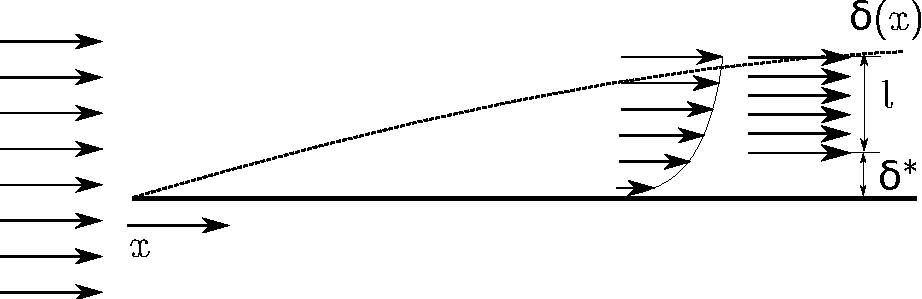
\includegraphics[width=0.8\textwidth]{clase04/espesor_desplazamiento.pdf}
\caption{Espesor de desplazamiento.}
\label{fig:espesor_desplazamiento}
\end{figure}

Por otra parte, sabemos que para un flujo no viscoso, el caudal por unidad de ancho sería simplemente $Q_\text{NV} = U_\infty \cdot l$, donde $l$ es el alto de la sección transversal.
Para que $Q=Q_\text{NV}$, $l=Q/U_\infty$, y sabemos que $\delta^*=\delta-l$, por lo tanto
%
\begin{equation}
\delta^* = \delta - l = \delta - \int_0^\delta \frac{u(y)}{U_\infty}\mathrm{d}y.
\end{equation}
%
Podemos reescribir $\delta = \int_0^\delta 1\mathrm{d}y$, y reemplazando en la última ecuación llegamos a la siguiente expresión para $\delta^*$
%
\begin{equation}\label{eq:espesor_desplazamiento}
\delta^* = \int_0^\delta \left(1-\frac{u(y)}{U_\infty}\right)\mathrm{d}y
\end{equation}

\subsection*{Espesor de momentum}
\paragraph*{Flujo de momentum sobre una placa.}
La placa de la Figura \ref{fig:capa_limite} es suficientemente delgada como para no bloquear el flujo, sin embargo, la condición de deslizamiento hace que la velocidad sea cero sobre la placa, afectando el perfil de velocidad.
Hagamos un análisis integral de la cantidad de movimiento como lo que hacíamos en el curso anterior.
%
\begin{figure}[!h]
\centering
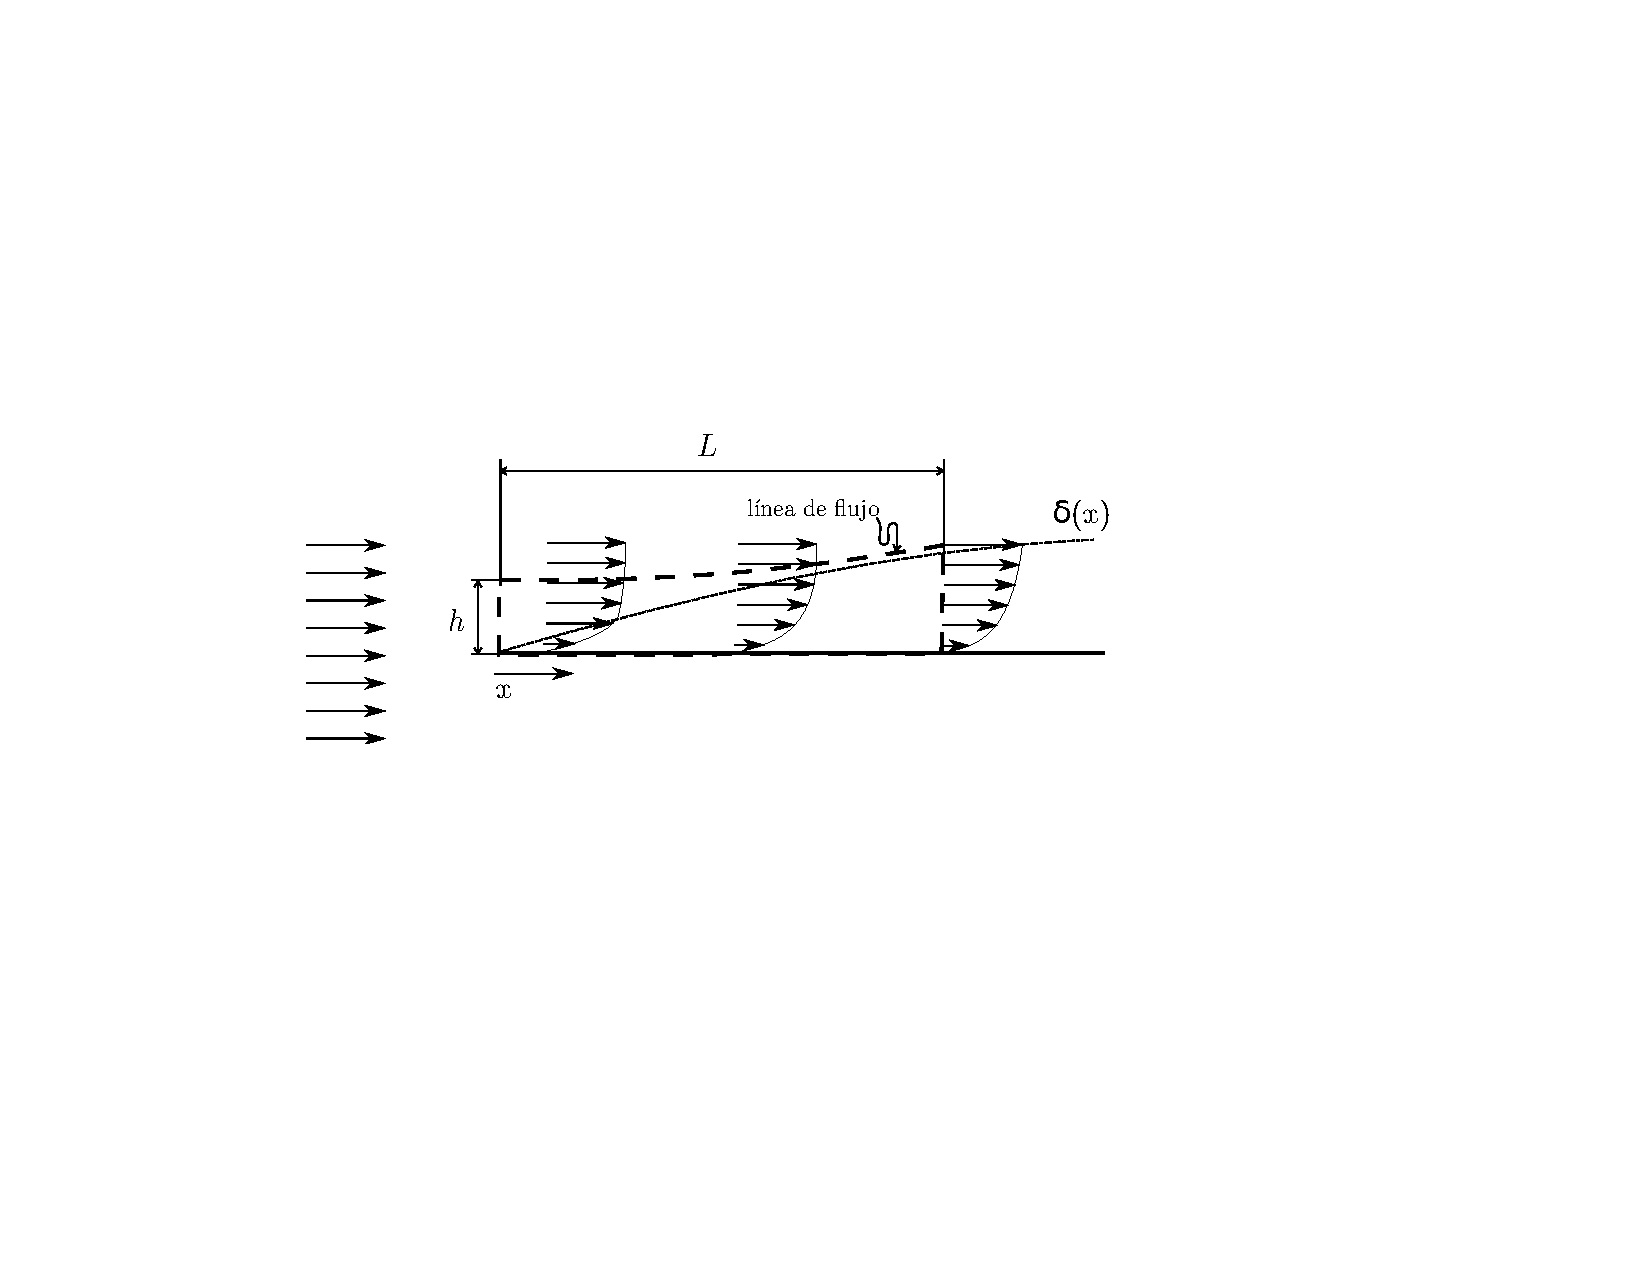
\includegraphics[width=0.8\textwidth]{clase04/analisis_integral.pdf}
\caption{Volúmen de control para análisis integral.}
\label{fig:analisis_integral}
\end{figure}
%
Elijamos el volumen de control que muestra la Figura \ref{fig:analisis_integral}, donde la parte de abajo está justo sobre la placa, el lado derecho va desde la placa hasta el fin de la capa límite $\delta(x)$, la línea superior coincide con una línea de flujo, y el lado izquierdo tiene altura $h$.
Recordando el análisis integral de la cantidad de movimiento, la ecuación para la fuerza en el eje $x$ es
%
\begin{equation}
\sum F_x = \frac{\partial}{\partial t} \int_{\vol} u\rho \mathrm{d}\vol + \oint_{\partial\vol} u\rho\mathbf{V}\cdot\mathbf{n}\mathrm{d}S.
\end{equation}
%
Consideremos un flujo externo con velocidad constante, y sin gradientes de presión. En este caso, la única fuerza es debido a la condición de no delizamiento. Además, el primer término de acumulación es cero, no pasa flujo ni por abajo (pared) ni por arriba (línea de flujo), y considerando que el flujo a la entrada es constante $U_\infty$, llegamos a
%
\begin{equation}\label{eq:capa_limite_momentum1}
F_x = -\rho U_\infty^2 bh + \rho b \oint_0^\delta u^2\mathrm{d}y.
\end{equation}
%
También, el principio de continuidad nos dice que todo lo que entra por la izquierda, sale por la derecha
%
\begin{align}\label{eq:capa_limite_cont}
\rho U_\infty bh &= \rho b \int_0^\delta u(y)\mathrm{d}y \nonumber\\
\Rightarrow U_\infty h &= \int_0^\delta u(y)\mathrm{d}y.
\end{align}
%
Reemplazando la Ec. \eqref{eq:capa_limite_cont} en la Ec. \eqref{eq:capa_limite_momentum1}, podemos reescribir la Ec. \eqref{eq:capa_limite_momentum1} como
%
\begin{equation}\label{eq:capa_limite_momentum}
D = -F_x = \rho b \oint_0^\delta u(U_\infty - u)\mathrm{d}y.
\end{equation}
%
donde $D$ es la fuerza sobre la placa.

\paragraph*{Espesor de momentum}
Como podemos imaginarnos, la fuerza sobre la placa depende del largo de esta (o el largo $L$ de la Figura \ref{fig:analisis_integral}), por lo tanto $D=D(x)$.
De aquí podemos definir el espesor de momentum ($\theta$) como:
%
\begin{equation}\label{eq:espesor_momentum}
\theta = \int_0^\delta \frac{u}{U_\infty}\left(1-\frac{u}{U_\infty}\right)\mathrm{d}y
\end{equation}
%
por lo tanto,
%
\begin{equation}\label{eq:D_momentum}
D(x) = \rho b U_\infty^2\theta.
\end{equation}

El espesor de momentum puede ser visto como la distancia que debemos mover la placa hacia arriba tal que un flujo no viscoso tuviese el mismo momentum.
Fíjense en la Ec. \eqref{eq:D_momentum}; ésta no es más que el flujo de momentum a través de un área de ancho $b$ y alto $\theta$ de un flujo uniforme, igualado a la fuerza sobre la placa.
Considerando que la fuerza sobre la placa debe ser igual al flujo de momentum de la capa límite, $\theta$ es un altura tal que los flujos de momentum del caso viscoso y no viscoso, sean iguales.

\section*{Espesor de capa límite laminar sin gradiente de presión}

\subsection*{El análisis de von Kármán}
\paragraph*{La relación integral de momentum.}

Quizás la forma más fácil de encontrar una expresión para el espesor de capa límite $\delta$ es a través de un análisis de cantidad de movimiento de la placa.
De hecho, la clase pasada hicimos este análisis para el caso particular en que la velocidad fuera de la capa límite $U_\infty$ sea independiente de $x$, y llegamos a
%
\begin{align}
D(x) &= \rho bU_\infty^2\theta\text{, con el espesor de momentum,}\nonumber\\
\theta &= \int_0^\delta\frac{u(y)}{U_\infty}\left(1-\frac{u(y)}{U_\infty}\right)\mathrm{d}y
\end{align}

De no ser $U_\infty$  independiente de $x$, por Bernoulli podemos darnos cuenta que habría un gradiente de presión, y considerando que $dp/dy=0$ dentro de la capa límite, tendríamos que sumar la contribución de este $\Delta p$ a la suma de fuerzas.
De este caso ya hablaremos más adelante.

La fuerza sobre la placa $D(x)$ es el resultado de esfuerzos cortantes ($\tau_w$) a lo largo de la placa.
Matemáticamente, esto es
%
\begin{equation}
D(x) = b\int_0^x \tau_w(x)\mathrm{d}x,
\end{equation}
%
lo que implica que
%
\begin{align}\label{eq:tau_w}
\frac{dD}{dx}=b\tau_w \text{ y, }\nonumber\\
\tau_w=\rho U_\infty^2 \frac{d\theta}{dx}.
\end{align}
%
Esta última relación se conoce como la relación integral de momentum para flujo en la capa límite sobre una placa plana.

\paragraph*{Espesor de capa límite de von Kármán.}
Para obtener una expresión de $\delta(x)$, von Kármán asumió un perfil de velocidad con forma parabólica:
%
\begin{equation}\label{eq:perfil_vk}
u(x,y) = U_\infty\left(\frac{2y}{\delta}-\frac{y^2}{\delta^2}\right) \quad 0\leq y\leq \delta(x).
\end{equation}
%
Reemplazando la Ec. \eqref{eq:perfil_vk} en el espesor de momentum $\theta$, llegamos a
%
\begin{equation}\label{eq:espesor_mom_vk}
\theta = \int_0^\delta \left(\frac{2y}{\delta} - \frac{y^2}{\delta^2}\right)\left(1-\frac{2y}{\delta} + \frac{y^2}{\delta^2}\right)\mathrm{d}y=\frac{2}{15}\delta.
\end{equation}
%
Podemos también calcular $\tau_w$ usando:
%
\begin{equation}\label{eq:tau_w2}
\tau_w = \mu\frac{du}{dy} = 2\frac{\mu U_\infty}{\delta}.
\end{equation}
%
Reemplazando la relación integral de momentum (Ec. \eqref{eq:tau_w}) en la Ec. \eqref{eq:tau_w2}, y usando la Ec. \eqref{eq:espesor_mom_vk} llegamos a una expresión para $\delta$:
%
\begin{align}
2\frac{\mu U_\infty}{\delta} &= \rho U_\infty^2 \frac{d\theta}{dx} = \rho U_\infty^2 \frac{2}{15}\frac{d\delta}{dx}\nonumber\\
\Rightarrow \delta d\delta &= 15\frac{\nu}{U_\infty}dx
\end{align}
% 
e integrando esta última expresión, tomando en cuenta que $\delta=0$ para $x=0$, obtenemos:
%
\begin{align}\label{eq:delta_vk}
\frac{1}{2}\delta^2 &= 15 \frac{\nu x}{U_\infty} \nonumber\\
\Rightarrow \frac{\delta}{x} &= 5.5\left(\frac{\nu}{U_\infty x}\right)^{1/2} = \frac{5.5}{\sqrt{Re_x}}.
\end{align}
%
Como adelantamos al principio de la clase, obtuvimos una expresión en función de $Re_x$.

Por otra parte, podemos también calcular el coeficiente de arrastre local $c_f$ como:
%
\begin{equation}\label{eq:cf_vk}
c_f = \frac{\tau_w}{\frac{1}{2}\rho U_\infty^2} = 4\frac{1}{\rho U_\infty^2}\frac{\mu U_\infty}{\delta} = \frac{0.73}{\sqrt{Re_x}}
\end{equation}
%
y el espesor de desplazamiento:
%
\begin{align}\label{eq:desplazamiento_vk}
\delta^* &= \int_0^\delta\left(1-\frac{u}{U_\infty}\right)\mathrm{d}y = \int_0^\delta \left(1-\frac{2y}{\delta}+\frac{y^2}{\delta^2}\right)\nonumber\\
&= \left. y-\frac{y^2}{\delta}+\frac{y^3}{3\delta}\right/_0^\delta = \frac{\delta}{3}\nonumber\\
\Rightarrow \frac{\delta^*}{x} &= \frac{1.83}{\sqrt{Re_x}}
\end{align}

Los valores de espesor de capa límite obtenidos con el análisis de von Kármán dependen de la aproximación que la velocidad dentro de la capa límite tiene forma parabólica. 
En la realidad, esto no es así, sin embargo los valores de $\delta$, $\delta^*$, $c_f$, $\tau_w$ y $\theta$ dados por este análisis hacen buenas predicciones y, en general, están a menos de un 10\% del valor real.




 
\end{document}
